\chapter{SCStack}
\label{chap:scstack}

\par SCStack es el conjunto de herramientas que componen la Forja de desarrollo. La palabra \emph{stack} en Inglés significa \emph{pila}, con respecto a la forja se trata del conjunto de herramientas apiladas y conectadas que dan forma a la Forja.

\begin{figure}[H]
    \centering
    
\includegraphics[width=0.7\textwidth]{stackstorage}
    \caption{Ejemplo de pila a partir de cajones}
    \label{fig:stackstorage}
\end{figure}

\section{Arquitectura}
\label{sec:arquitectura}

\par La arquitectura del Sistema de Gestión de la Forja se ve reflejada en el siguiente esquema:

% TODO Imagen UI -> REST Server -> API

\par El proyecto consta de tres componentes conectados entre sí para la comunicación del usuario con las herramientas para la gestión de los proyectos: La Consola de Administración, el servidor de servicios web REST y el API.

\subsection{Consola de Administración}
\label{sub:consola-admin}

\par \textbf{Consola de Administración}: Se trata de la capa de la vista encargada de interactuar con el usuario. A través de la interfaz que se ejecuta sobre un navegador web, el usuario administrador gestiona los usuarios y los proyectos de la Forja: crear, editar, modificar, eliminar y buscar), el típico sistema CRUD-F\footnote{\url{http://en.wikipedia.org/wiki/Create,\_read,\_update\_and\_delete}} (\emph{CRUD: Create, Read, Update and Delete also Find}). Está diseñada con el framework Javascript \emph{jQuery} por lo que no requiere ninguna librería externa para su uso, únicamente el navegador del cliente. Las operaciones que se realizan en la capa UI se trasladan al servidor REST a través de peticiones \emph{http} asíncronas mediante las interfaces REST definidas.

% subsection consola-admin (end)

\subsection{Servicio web REST}
\label{sub:rest-ws}

\par \emph{REST}: Representational State Transfer se trata de una arquitectura acuñada por \emph{Roy Fielding}\footnote{\url{http://roy.gbiv.com/}}, uno de los autores de la especificación del protocolo \emph{HTTP}. Esta arquitectura de comunicación se basa en cuatro principios:

\begin{itemize}
	\item Un protocolo cliente/servidor \emph{sin estado}: cada mensaje HTTP contiene toda la información necesaria para comprender la petición. Como resultado, ni el cliente ni el servidor necesitan recordar ningún estado de las comunicaciones entre mensajes. Sin embargo, en la práctica, muchas aplicaciones basadas en HTTP utilizan cookies y otros mecanismos para mantener el estado de la sesión.

	\item Un \emph{conjunto de operaciones} bien definidas que se aplican a todos los recursos de información: HTTP en sí define un conjunto pequeño de operaciones, las más importantes son \textbf{POST}, \textbf{GET}, \textbf{PUT} y \textbf{DELETE}.

	\item Una sintaxis \emph{universal} para identificar los recursos. En un sistema REST, cada recurso es direccionable únicamente a través de su URI.

	\item El uso de \emph{hipermedios}: tanto para la información de la aplicación como para las transiciones de estado de la aplicación. Como resultado de esto, es posible navegar de un recurso REST a muchos otros, simplemente siguiendo enlaces sin requerir el uso de registros u otra infraestructura adicional.
\end{itemize}

\par El uso de los servicios REST para la comunicación mediante el protocolo http con la Consola de Administración agiliza la adaptación de la funcionalidades al cliente, el tráfico y las posibles adaptaciones de nuevos clientes para el acceso a través de cualquier plataforma.

\begin{figure}[H]
    \centering
    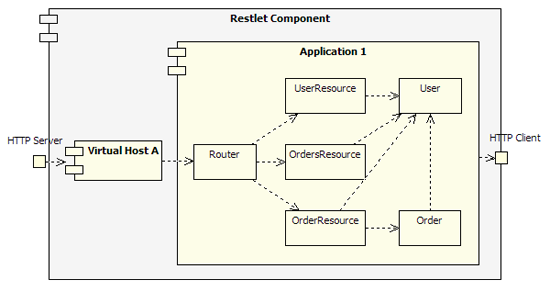
\includegraphics[width=1\textwidth]{restlet}
    \caption{Diseño de un API RESTful}
    \label{fig:restful-api}
\end{figure}

\par \textbf{Servicio web REST}: Es el componente encargado de gestionar las peticiones http a los servicios REST de la Consola de Administración y el API de SidelabCode. Define e implementa la lógica a seguir para la construcción de un proyecto a través de la UI mediante las llamadas ordenadas al API de cada una de las herramientas involucradas en el servicio como componentes de la forja.

\par Los servicios REST ofrecen tres interfaces distintas accesibles a través de http: XML, JSON y HTML para la comunicación la API. Además, hay que desatacar que el servicio web es servido a través del framework \emph{Restlet} a través de Internet de forma continua y remota a cualquier usuario o proceso cliente.

\par Se encarga de la seguridad y validación para las operaciones permitidas o denegadas del usuario de la UI, proporcionando, según su rol, determinados servicios a través de la Consola de Administración, buscar proyectos, crear usuarios, editar proyectos, crear proyectos, etc.

% subsection rest-ws (end)

\subsection{API}
\label{sub:api}

\par \textbf{API}: La API es el núcleo funcional de SCStack, coordina y realiza las tareas para cada componente de la forja con respecto a los usuarios y proyectos involucrados. Traslada las órdenes ejecutadas en la capa UI a las distintas herramientas para configurar su funcionamiento. Está conectada a todos los servicios que ofrece pivotando a través del directorio LDAP: Control de Versiones, Directorios, Integración Continua, ITS, Revisiones, Gestión de Dependencias, Seguridad y Autenticación que analizaremos extensamente más adelante componente a componente.

% subsection api (end)

% section arquitectura (end)

\section{Provisionamiento (puppet)}
\label{sec:puppet}

% section puppet (end)

\section{Componentes}
\label{sec:componentes}

\begin{comment}
Componentes, ¿ aquí se definirían las herramientas a instalar ?

Efectivamente, qué herramientas instala la forja (Se supone que las has descrito en la parte de procesos de desarrollo de forma genérica, aquí se dan nombres concretos). 
\end{comment}

\par En este apartado se van a analizar las distintas partes o componentes que integran la Forja SidelabCode Stack y el papel que desempeñan en el funcionamiento del sistema. Partiendo del esquema en donde se refleja a grandes rasgos la arquitectura de la Forja SidelabCode.

\begin{itemize}
	\item Gesti\'on de Requisitos.
	\item Arquitectura.
	\item Desarrollo.
	\item Test.
	\item Issue tracking system.
	\item Continuous Integration.
	\item Release Management.
\end{itemize}

% subsection componentes (end)

\section{Interoperabilidad}
\label{sec:interoperabilidad}

\par Interoperabilidad entre las herramientas que componen la forja. API Rest.

% section interoperabilidad (end)

\section{Pruebas y Validación}
\label{sec:pruebas-validacion}

\par Pruebas a trav\'es de virtualizaci\'on de sistemas operativos mediante herramientas libres; Vagrant, kvm, puppet.

% section pruebas-validacion (end)
